%----------------------------------------------------------------------------------------------------------------
% Apostila LaTeX
% Codificação: UTF-8
% LaTeX:  abnTeX2
% ---------------------------------------------------------------------------------------------------------------

% CARREGA CLASSE PERSONALIZADA COM AS NORMAS DA URI-----------------------------------------------------------
\documentclass[oneside]{template-config/uri-abntex2}

% INCLUI ARQUIVOS DE CONFIGURAÇÕES-------------------------------------------------------------------------------
% REFERÊNCIAS------------------------------------------------------------------
\usepackage[%
    alf,
    abnt-emphasize=bf,
    bibjustif,
    recuo=0cm,
    abnt-url-package=url,       % Utiliza o pacote url
    abnt-refinfo=yes,           % Utiliza o estilo bibliográfico abnt-refinfo
    abnt-etal-cite=3,
    abnt-etal-list=3,
    abnt-thesis-year=final
]{abntex2cite}                  % Configura as citações bibliográficas conforme a norma ABNT

% PACOTES----------------------------------------------------------------------
\usepackage[utf8]{inputenc}                                 % Codificação do documento
\usepackage[T1]{fontenc}                                    % Seleção de código de fonte
\usepackage{booktabs}                                       % Réguas horizontais em tabelas
\usepackage{color, colortbl}                                % Controle das cores
\usepackage{float}                                          % Necessário para tabelas/figuras em ambiente multi-colunas
\usepackage{graphicx}                                       % Inclusão de gráficos e figuras
\usepackage{icomma}                                         % Uso de vírgulas em expressões matemáticas
\usepackage{indentfirst}                                    % Indenta o primeiro parágrafo de cada seção
\usepackage{microtype}                                      % Melhora a justificação do documento
\usepackage{multirow, array}                                % Permite tabelas com múltiplas linhas e colunas
\usepackage{subeqnarray}                                    % Permite subnumeração de equações
\usepackage{lastpage}                                       % Para encontrar última página do documento
\usepackage{verbatim}                                       % Permite apresentar texto tal como escrito no documento, ainda que sejam comandos Latex
\usepackage{amsfonts, amssymb, amsmath}                     % Fontes e símbolos matemáticos
\usepackage[algoruled, portuguese]{algorithm2e}             % Permite escrever algoritmos em português
%\usepackage[scaled]{helvet}                                % Usa a fonte Helvetica
\usepackage{times}                                          % Usa a fonte Times
%\usepackage{palatino}                                      % Usa a fonte Palatino
%\usepackage{lmodern}                                       % Usa a fonte Latin Modern
\usepackage[bottom]{footmisc}                               % Mantém as notas de rodapé sempre na mesma posição
\usepackage{ae, aecompl}                                    % Fontes de alta qualidade
\usepackage{latexsym}                                       % Símbolos matemáticos
\usepackage{lscape}                                         % Permite páginas em modo "paisagem"
%\usepackage{picinpar}                                      % Dispor imagens em parágrafos
%\usepackage{scalefnt}
\usepackage{setspace}                                    % Permite redimensionar tamanho da fonte
%\usepackage{subfig}                                        % Posicionamento de figuras
%\usepackage{upgreek}                                       % Fonte letras gregas

% Redefine a fonte para uma fonte similar a Arial (fonte Helvetica)
% \renewcommand*\familydefault{\sfdefault}
% Configura todo o documento para times new roman
\renewcommand{\familydefault}{ptm}

% CONFIGURAÇÕES DE APARÊNCIA DO PDF FINAL--------------------------------------
\makeatletter
\hypersetup{%
    portuguese,
    colorlinks=true,   % true: "links" coloridos; false: "links" em caixas de texto
    linkcolor=black,    % Define cor dos "links" internos
    citecolor=black,    % Define cor dos "links" para as referências bibliográficas
    filecolor=black,    % Define cor dos "links" para arquivos
    urlcolor=black,     % Define a cor dos "hiperlinks"
    breaklinks=true,
    pdftitle={\@title},
    pdfauthor={\@author},
    pdfkeywords={abnt, latex, abntex, abntex2}
}
\makeatother

% ALTERA O ASPECTO DA COR AZUL--------------------------------------------------
\definecolor{blue}{RGB}{41,5,195}

% REDEFINIÇÃO DE LABELS---------------------------------------------------------
\renewcommand{\algorithmautorefname}{Algoritmo}
\def\equationautorefname~#1\null{Equa\c c\~ao~(#1)\null}

% CRIA ÍNDICE REMISSIVO---------------------------------------------------------
\makeindex

% HIFENIZAÇÃO DE PALAVRAS QUE NÃO ESTÃO NO DICIONÁRIO---------------------------
\hyphenation{%
    qua-dros-cha-ve
    Kat-sa-gge-los
}



% INCLUI ARQUIVOS DO TRABALHO DE CONCLUSÃO DE CURSO (PRÉ-TEXTUAIS, TEXTUAIS, PÓS-TEXTUAIS)-----------------------

% INSERE CAPA E FOLHA DE ROSTO
% CAPA---------------------------------------------------------------------------------------------------

% ORIENTAÇÕES GERAIS-------------------------------------------------------------------------------------
% Caso algum dos campos não se aplique ao seu trabalho, como por exemplo,
% se não houve coorientador, apenas deixe vazio.
% Exemplos: 
% \coorientador{}
% \departamento{}

% DADOS DO TRABALHO--------------------------------------------------------------------------------------
\titulo{Título do Trabalho: Subtítulo do Trabalho}
% \titleabstract{Title in English}
\autor{Nome Completo do Autor}
% \autorcitacao{SOBRENOME, Nome} % Sobrenome em maiúsculo
\local{ERECHIM - RS}
\data{2018}

% NATUREZA DO TRABALHO-----------------------------------------------------------------------------------
% Opções: 
% - Projeto de Conclusão de Curso (Disciplina de Projeto)
% - Trabalho de Conclusão de Curso (se for Graduação)
% - Dissertação (se for Mestrado)
% - Tese (se for Doutorado)
% - Projeto de Qualificação (se for Mestrado ou Doutorado)
% \projeto{Trabalho de Conclusão de Curso}

% TÍTULO ACADÊMICO---------------------------------------------------------------------------------------
% Opções:
% - Bacharel ou Tecnólogo (Se a natureza for Trabalho de Conclusão de Curso)
% - Mestre (Se a natureza for Dissertação)
% - Doutor (Se a natureza for Tese)
% - Mestre ou Doutor (Se a natureza for Projeto de Qualificação)
% \tituloAcademico{Bacharel}

% ÁREA DE CONCENTRAÇÃO E LINHA DE PESQUISA---------------------------------------------------------------
% Se a natureza for Trabalho de Conclusão de Curso, deixe ambos os campos vazios
% Se for programa de Pós-graduação, indique a área de concentração e a linha de pesquisa
% \areaconcentracao{}
% \linhapesquisa{}

% DADOS DA INSTITUIÇÃO-----------------------------------------------------------------------------------
% Se a natureza for Trabalho de Conclusão de Curso, coloque o nome do curso de graduação em "programa"
% Formato para o logo da Instituição: \logoinstituicao{<escala>}{<caminho/nome do arquivo>}
% \instituicao{Universidade Regional Integrada do Alto Uruguai e das Missões Campus de Erechim}
% \departamento{Departamento de Engenharias e Ciência da Computação}
% \programa{Curso de Ciência da Computação}
% \disciplina{Projeto de Conclusão de Curso}
%\logoinstituicao{0.2}{dados/figuras/logo-instituicao.png} 

% DADOS DOS ORIENTADORES---------------------------------------------------------------------------------
% \orientador{Nome do orientador}
%\orientador[Orientadora:]{Nome da orientadora}
% \instOrientador{Instituição do orientador}

% \coorientador{Nome do coorientador}
%\coorientador[Coorientadora:]{Nome da coorientadora}
% \instCoorientador{Instituição do coorientador}


\begin{document}

\pretextual
\imprimircapa                                               	               % Comando para imprimir Capa
% \imprimirfolhaderosto{}                                     		           % Comando para imprimir Folha de rosto
% \imprimirfolhadeaprovacao
% INSERE ELEMENTOS PRÉ-TEXTUAIS     			           
% Lista de Figuras----------------------------------------------------------------

\pdfbookmark[0]{\listfigurename}{lof}
\listoffigures*
\cleardoublepage

% OBSERVAÇÕES---------------------------------------------------------------------
% Este arquivo não precisa de ser alterado, pois a lista é gerada automaticamente.
   % Lista de Figuras
% LISTA DE QUADROS----------------------------------------------------------------

\renewcommand{\listofquadrosname}{LISTA DE QUADROS}

\pdfbookmark[0]{\listofquadrosname}{loq}
\listofquadros*
\cleardoublepage

% OBSERVAÇÕES---------------------------------------------------------------------
% Este arquivo não necessita de ser editado. A lista é gerada automaticamente.
   % Lista de Quadros
% LISTA DE TABELAS-------------------------------------------------------------

\pdfbookmark[0]{\listtablename}{lot}
\listoftables*
\cleardoublepage

% OBSERVAÇÕES-------------------------------------------------------------------
% Este arquivo não precisa ser alterado, pois a lista é gerada automaticamente.
         		       % Lista de Tabelas
% LISTA DE ABREVIATURAS E SIGLAS----------------------------------------------------------

\begin{siglas}
    \item[ABNT] Associação Brasileira de Normas Técnicas
    \item[DECOM] Departamento de Computação
\end{siglas}

% OBSERVAÇÕES-----------------------------------------------------------------------------
% Altere a lista acima para definir os acrônimos e siglas utilizados neste trabalho
          		       % Lista de Abreviaturas e Siglas
% LISTA DE SÍMBOLOS------------------------------------------------------------

\begin{simbolos}
    \item[$ \Gamma $] Letra grega Gama
    \item[$ \lambda $] Comprimento de onda
    \item[$ \in $] Pertence
\end{simbolos}

% OBSERVAÇÕES-------------------------------------------------------------------
% Altere a lista acima para definir os símbolos utilizados no trabalho
        		       % Lista de Símbolos
% LISTA DE ALGORITMOS----------------------------------------------------------

\newcommand{\algoritmoname}{Algoritmo}
\renewcommand{\listalgorithmcfname}{LISTA DE ALGORITMOS}

\floatname{algocf}{\algoritmoname}
\newlistof{listofalgoritmos}{loa}{\listalgoritmoname}
\newlistentry{algocf}{loa}{0}

\counterwithout{algocf}{chapter}
\renewcommand{\cftalgocfname}{\algoritmoname\space}
\renewcommand*{\cftalgocfaftersnum}{\hfill--\hfill}

\pdfbookmark[0]{\listalgorithmcfname}{loa}
\listofalgorithms
\cleardoublepage

% OBSERVAÇÕES------------------------------------------------------------------
% Este arquivo não precisa ser alterado, pois a lista é gerada automaticamente.
   % Lista de Algoritmos
% SUMÁRIO----------------------------------------------------------------------

\renewcommand{\contentsname}{SUMÁRIO}

\pdfbookmark[0]{\contentsname}{toc}
\tableofcontents*
\cleardoublepage               			           % Sumário

\textual
% INSERE ELEMENTOS TEXTUAIS
% INTRODUÇÃO-------------------------------------------------------------------

\chapter{INTRODUÇÃO}
\label{chap:introducao}

\LaTeX{} é um conjunto de macros de alto nível para \TeX \xspace que torna mais fácil e rápida a produção de todo o tipo de documentos como, por exemplo, livros, relatórios e artigos.

O objetivo do \LaTeX \xspace é que o autor se possa distanciar da apresentação visual do trabalho e assim se concentrar no seu conteúdo. Possui formas de lidar com bibliografias, citações, formatos de páginas, referências e tudo mais que não seja relacionado com conteúdo do documento em si.

\section{Histórico}
\label{sec:Histórico}

Em 1978 Donald E. Knuth começou a desenvolver uma linguagem cujo objetivo era permitir a qualquer um formatar textos com muitas equações e com alta qualidade de saída, chamada de \TeX. Em 1985 Leisle Lamport desenvolveu um conjunto de macros denominado \LaTeX \xspace, que simplifica o uso da linguagem \TeX \xspace. Atualmente este projeto é mantido e desenvolvido pelo \LaTeX3 \xspace Project

O som final dos nomes \TeX \xspace e \LaTeX \xspace deve ser pronunciado como se fosse um “K”.

\section{Instalação}
\label{sec:Instalação}

\LaTeX é um software livre e gratuito, é possível instalar nos  principais sistemas operacionais modernos como: Windows 7, 8, 8.1 e 10; Mac OS e várias distribuições Linux.

\subsection{Windows}

MiKTeX é uma distribuição TeX / LaTeX para o Microsoft Windows. Baixe o instalador pelo link oficial: \href{https://miktex.org/download}{\textcolor{blue}{Download MiKTeX}}

A instalação do MiKTeX é simples, basicamente é só clicar no “Avançar”. Caso houver problemas na instalação o seguinte vídeo poderá servir de ajuda: \href{https://www.youtube.com/watch?v=4udFXbqtayE&list=LLQVoeslEpxQJ0UavpXUEkq}{\textcolor{blue}{Vídeo Instalação MiKTeX}}. Junto com a instalação do MiKTeX o editor TeXworks é instalado. Existem outros editores como o Texmaker. 

O Texmaker é mais simples de usar e é o editor de código aberto mais popular entre a comunidade LaTeX. Baixe o instalador pelo link oficial: \href{http://www.xm1math.net/texmaker/download.html}{\textcolor{blue}{Download TeXMaker}}

\subsection{Ubuntu}

O TeX Live é uma distribuição para produção de documentos \TeX \xspace. Para instalar no ubuntu 16.04 digite o seguinte comando: 
\begin{lstlisting}[language=bash]
    $ sudo apt-get install texlive-full
\end{lstlisting}

Apos a instalação do TeX Live pode-se obtar por instalar um editor específico para LaTeX o Texmaker, para instalar digite o seguinte comando: 

\begin{lstlisting}[language=bash]
    $ sudo apt-get install texmaker
\end{lstlisting}

\section{Compilação Tex Maker}

Para Compilar o arquivo \emph{.tex} junto com o arquivo \emph{.bib} no TeX Maker é necessário uma configuração, como mostra as Figuras \ref{fig:texmaker-config1} e \ref{fig:texmaker-config2}.

\begin{figure}[H]
    \centering
    \caption{Configuração Tex Maker}
    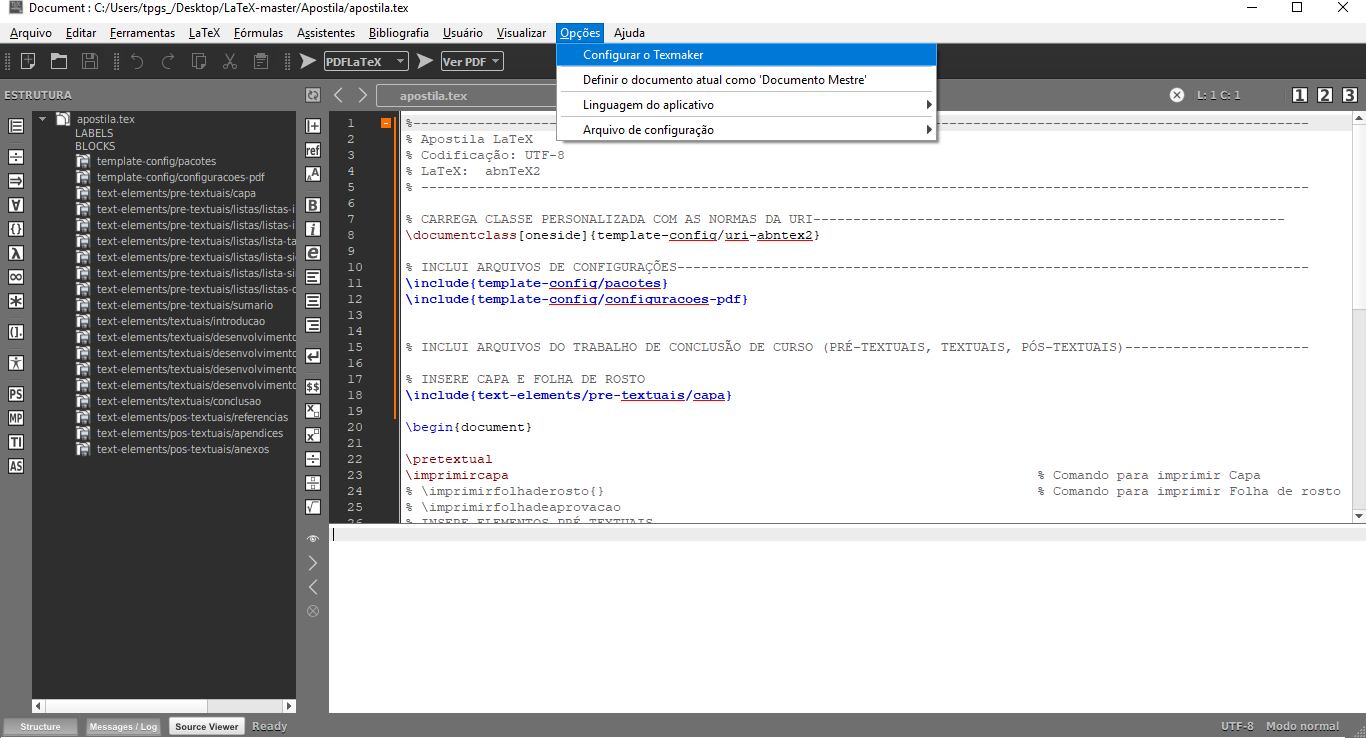
\includegraphics[width=0.70\textwidth]{./dados/figuras/compiler1}
    \fonte{Autor}
    \label{fig:texmaker-config1}
\end{figure}

\begin{figure}[H]
    \centering
    \caption{Configuração Tex Maker 2}
    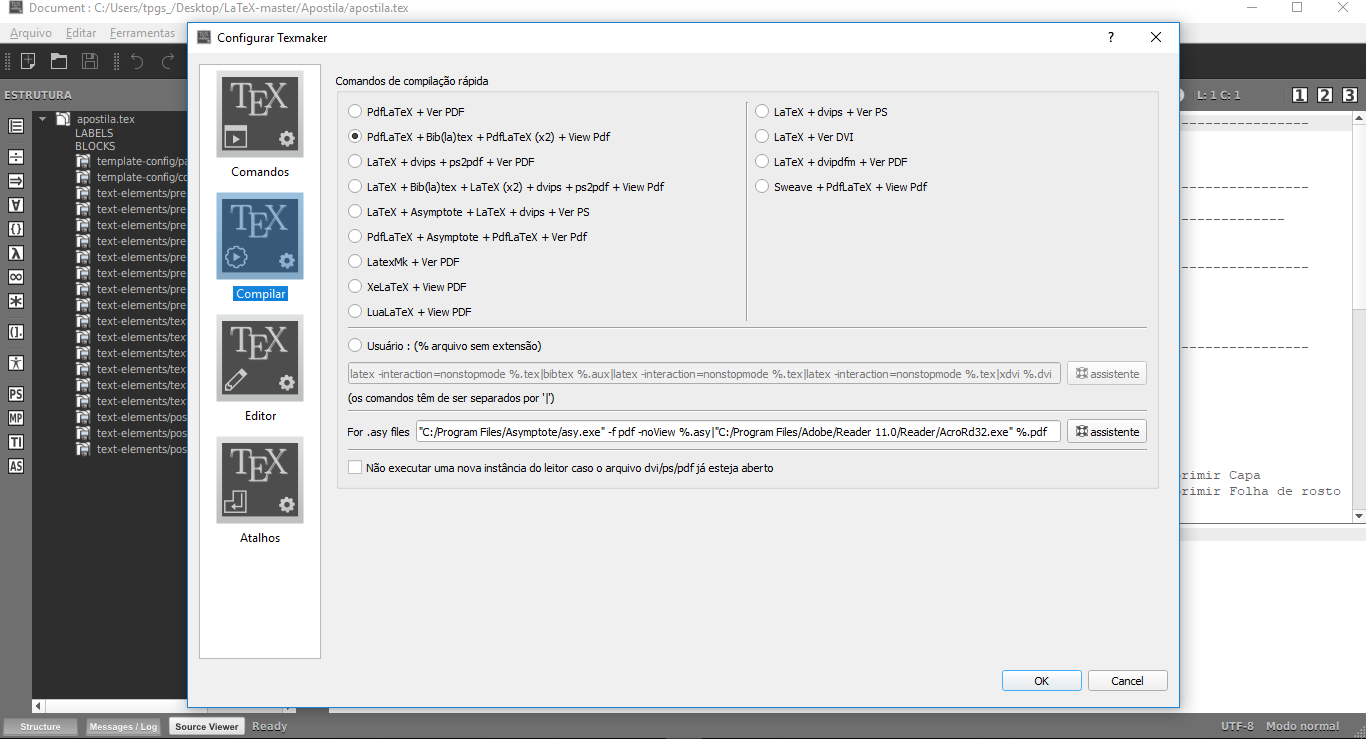
\includegraphics[width=0.70\textwidth]{./dados/figuras/compiler2}
    \fonte{Autor}
    \label{fig:texmaker-config2}
\end{figure}

\section{Compilação por Linha de Comando}

Para compilar pela linha de comando (windows e Linux) deve-se fazer os seguintes passos:

\begin{enumerate}
    \item Compilar o arquivo principal \emph{.tex}:
    \begin{lstlisting}[language=bash]
        pdflatex apostila.tex
    \end{lstlisting}
    \item Montar os índices:
    \begin{lstlisting}[language=bash]
        makeindex apostila.idx
    \end{lstlisting}
    \item Compilar o arquivo das bibliografias \emph{.bib}
    \begin{lstlisting}[language=bash]
        bibtex apostila.aux
    \end{lstlisting}
    \item Por fim, gerar o PDF:
    \begin{lstlisting}[language=bash]
        pdflatex apostila.tex
    \end{lstlisting}
\end{enumerate}

\section{Ferramentas em Nuvem}

Existem ferramentas que possibilitam a edição e a colaboração online de documentos LaTeX. Uma dessas ferramentas é o \href{https://www.overleaf.com/}{\textcolor{blue}{Overleaf}}.

Para usar o Overleaf basta criar uma conta, começar um projeto e escrever. Uma outra grande vantagem do Overleaf é a comunidade que compartilha templates prontos, como por exemplo:  \href{https://www.overleaf.com/latex/templates}{\textcolor{blue}{principais templates}}.                 		               % Introdução
% ESTRUTURA E COMANDOS--------------------------------------------------------

\chapter{ESTRUTURA E COMANDOS}
\label{chap:estruturaecomandos}

Um documento em \LaTeX{} começa pelo comando \verb|\documentclass[opcionais]{classe}|.
Abaixo desse comando são declarados os pacotes e outras configurações do documento.

Os comandos \verb|\begin{document}| e \verb|\end{document}| marcam o início do ambiente onde por exemplo,
as seções, subseções e o texto do documento serão inseridos. 
O seguinte trecho de código exemplifica a estrutura básica de um documento em \LaTeX.

\begin{verbatim}
\documentclass[opcionais]{classe}

    % declarações

\begin{document}

    % documento

\end{document}
\end{verbatim}

As principais\footnote{pode se encontrar encontrar outros parâmetros para classes e opções nesse link:
\href{https://en.wikibooks.org/wiki/LaTeX/Document_Structure}{\textcolor{blue}{Classes e Opções}}} 
classes que podem ser passadas para o comando \verb|\documentclass| são:\\

\begin{itemize}
    \item \{article\} - para produzir artigos curtos;
    \item \{report\} - para produzir artigos mais longos, relatórios e monografias;
    \item \{book\} - para produzir livros.\\
\end{itemize}

Nas opções é possível utilizar os seguintes parâmetros:\\

\begin{itemize}
    \item 11pt - fonte de 11 pontos;
    \item 12pt - fonte de 12 pontos;
    \item twoside - imprime em ambos os lados da folha;
    \item twocolumn - produz o documento formatado em duas colunas;
\end{itemize}

% ESTRUTURA E COMANDOS - Trabalhando com Projetos Grandes--------------------

\section{Trabalhando com Projetos Grandes}

O comando \verb|\include{nome_do_arquivo}| inclui um arquivo ao documento principal.
Este comando deve ser usado quando existem capítulos com quantidades maiores de conteúdo.

% ESTRUTURA E COMANDOS - Parâmetros Obrigatórios e Opcionais-----------------

\section{Parâmetros Obrigatórios e Opcionais}

Os comandos em \LaTeX{} são precedidos por \textbackslash e seguidos por [ ] e/ou \{ \}, onde:\\

[ ] Parâmetros opcionais.

\{ \} Parâmetros Obrigatórios.

% ESTRUTURA E COMANDOS - Comentários-----------------------------------------

\section{Comentários}

Comentários em um documento \TeX{} são ignorados pelo compilador.
Para utilizar comentários ao longo do texto utilize \%

% ESTRUTURA E COMANDOS - Parágrafos------------------------------------------

\section{Parágrafos}

Para iniciar um novo parágrafo no \LaTeX{}, deve-se deixar uma linha em branco entre os textos.

% ESTRUTURA E COMANDOS - Espaços---------------------------------------------

\section{Espaços}

Para produzir espaço durante texto pode-se usar \verb|\space{}|.
O comando \textasciitilde{} produz um espaço que não pode ser divido em uma quebra de linha,
por exemplo um número de telefone: 54~11111-1111.

Ainda é possível utilizar o comando \verb|\vspace{espaço}| para colocar espaços verticais.
Assim como também é possível colocar espaços horizontais com o comando
\verb|\hspace{espaço}|.

Em {espaço} deve-se passar a quantidade do espaço desejado.
Pode-se usar as dimensões em pontos (pt), polegadas (in),
milímetros (mm), centímetros (cm) etc.            % Revisão de Literatura
% SIMBOLOS E ACENTUAÇÃO-------------------------------------------------------------------

\chapter{SIMBOLOS E ACENTUAÇÃO}

\TeX{} usa ASCII por padrão. Mas para que acentos e outros caracteres especiais apareçam diretamente no arquivo de origem,
deve-se dizer ao \TeX{} usar uma codificação diferente.


\LaTeX{} suporta a composição de caracteres especiais.
Isto é conveniente se o seu teclado não tiver alguns acentos desejados e outros diacríticos.

Os seguintes acentos podem ser colocados em letras.
Embora a letra 'o' seja usada na maioria dos exemplos, os acentos podem ser colocados em qualquer letra.
Os acentos podem até ser colocados acima de uma letra “ausente”; por exemplo, \verb|\ ~ {}| produz um til sobre um espaço em branco.

Para que a acentuação ocorra de forma automática deve-se usar os seguintes pacotes:

\begin{verbatim}
\usepackage[brazilian]{babel}
\usepackage[utf8]{inputenc}
\usepackage[T1]{fontenc}
\end{verbatim}

LaTeX tem muitos símbolos à sua disposição.
A maioria deles está no domínio matemático e os capítulos posteriores abordarão como obter acesso a eles.
Para os símbolos de texto mais comuns, use os seguintes comandos:

\begin{quadro}[!htb]
    \centering
    \caption{Exemplo Simbolos Especiais.\label{qua:quadro-simbolos-especiais}}
        \begin{tabular}{|l|l|l|}
            \hline
                \multicolumn{1}{|c|}{\textbf{Comando em \LaTeX{}}} & \multicolumn{1}{c|}{\textbf{Exemplo}} \\ \hline
                \verb|\$|                                       & \$                                     \\ \hline
                \verb|\&|                                       & \&                                      \\ \hline
                \verb|\%|                                       & \%                                       \\ \hline
        \end{tabular}
\end{quadro}
% ORIENTAÇÕES GERAIS------------------------------------------------------------

% QUADROS E TABELAS---------------------------------------------------------------
\chapter{QUADROS E TABELAS}
\label{chap:tabelas}

Formatar colunas no \LaTeX{} é um pouco mais trabalhoso. Porém, ambos aparecem automaticamente nas suas respectivas listas (indexações).
No caso deste template, ambos os elementos (Quadros e Tabelas) devem ser criados em arquivos separados para facilitar manutenção e armazenados no diretório de "/dados".

\begin{quadro}[!htb]
    \centering
    \caption{Exemplo de Quadro.\label{qua:quadro-exemplo1}}
    \begin{tabular}{|p{7cm}|p{7cm}|}
        \hline
        \textbf{BD Relacionais} & \textbf{BD Orientados a Objetos} \\
        \hline
        Os dados são passivos, ou seja, certas operações limitadas podem ser automaticamente acionadas quando os dados são usados. & Os processos que usam dados mudam constantemente. \\
        \hline
    \end{tabular}
    \fonte{\citeonline{Barbosa2004}}
\end{quadro}


\begin{table}[!htb]
    \centering
    \caption[Resultado dos testes]{Resultado dos testes.
    \label{tab:tabela-exemplo1}}
    \begin{tabular}{rrrrr}
        \toprule
            & Valores 1 & Valores 2 & Valores 3 & Valores 4 \\
        \midrule
            Caso 1 & 0,86 & 0,77 & 0,81 & 163 \\
            Caso 2 & 0,19 & 0,74 & 0,25 & 180 \\
            Caso 3 & 1,00 & 1,00 & 1,00 & 170 \\
        \bottomrule
    \end{tabular}
    \fonte{\citeonline{Barbosa2004}}
\end{table}


No caso deste template, ambos os elementos (Quadros e Tabelas) devem ser criados em arquivos separados para facilitar manutenção e armazenados no diretório de "/dados".

Para posicionar as tabelas no documento, existem alguns simbolos a serem utilizados. O \autoref{qua:quadro-floats} demonstra os símbolos denominados \textit{floats}. Eles tem como objetivo definir o posicionamento do elemento dentro do documento.

\begin{quadro}[H]
    \centering
    \caption{Posicionamento da Tabela no Corpo do Documento.\label{qua:quadro-floats}}
    \begin{tabular}{|p{4cm}|p{10cm}|}
        \hline
        \textbf{Símbolo} & \textbf{Descrição} \\
        \hline
        h & here. Posiciona o elemento aproximadamente no mesmo local de onde ele foi adicionado no texto fonte \\
        \hline
        t & top. Posiciona o elemento no topo da página \\
        \hline
        b & bottom. Posiciona o elemento no fim da página \\
        \hline
        p &	Posiciona o elemento em uma página exclusiva para elementos flutuantes (e.g. imagens, tabelas, quadros) \\
        \hline
        ! & important. Sobrescreve todos parâmetros internos do LaTeX, forçando o objeto a ficar na posição solicitada \\
        \hline
        H & Posiciona o elemento exatamente no mesmo lugar onde inserido no texto fonte \\
        \hline
    \end{tabular}
\end{quadro}

Para delimitar os espaços das colunas e suas respectivas divisões, os símbolos mais utilizados são demonstrados pelo \autoref{qua:quadro-colunas}.

\begin{quadro}[H]
    \centering
    \caption{Símbolos para Descrição das Colunas.\label{qua:quadro-colunas}}
    \begin{tabular}{|p{4cm}|p{10cm}|}
        \hline
        \textbf{Símbolo} & \textbf{Descrição} \\
        \hline
        l & Coluna justificada a esquerda \\
        \hline
        c & Coluna centralizada \\
        \hline
        r & Coluna justificada a direita \\
        \hline
        p{width*} & Coluna com texto em parágrafo, com texto verticalmente alinhado no topo \\
        \hline
        m{width*} & Coluna-parágrafo com texto alinhado no centro \\
        \hline
        b{width*} & Coluna-parágrafo com texto alinhado embaixo \\
        \hline
        | & Linha vertical \\
        \hline
        || & Duas linhas verticais \\
        \hline
    \end{tabular}
\end{quadro}

Por fim, existem alguns símbolos que precisamos utilizar para delimitar e formatar as informações contidas dentro das tabelas, conforme o \autoref{qua:quadro-dados} mostra.

\begin{quadro}[H]
    \centering
    \caption{Símbolos para Formatação dos Dados.\label{qua:quadro-dados}}
    \begin{tabular}{|p{4cm}|p{10cm}|}
        \hline
        \textbf{Símbolo} & \textbf{Descrição} \\
        \hline
        \verb|/&	Separador de colunas| \\
        \hline
        \verb|\\	Inicializa nova linha| \\
        \hline
        \verb|/\hline	Linha horizontal (e.g. ---)|
        \verb|\newline	Inicia uma nova linha dentro de uma coluna-parágrafo|
        \toprule	Adiciona linha no topo da tabela
        \midrule	Adiciona linha entre o cabeçalho da tabela e os dados
        \bottomrule	Adiciona linha no final da tabela\\
        \hline
    \end{tabular}
\end{quadro}

A diferença entre quadro e tabela está no fato que um quadro é formado por linhas horizontais e verticais. Deve ser utilizado quando o conteúdo é majoritariamente não-numérico. O número do quadro e o título vem acima do quadro, e a fonte, deve vir abaixo. E Uma tabela é formada apenas por linhas verticais. Deve ser utilizada quando o conteúdo é majoritariamente numérico. O número da tabela e o título vem acima da tabela, e a fonte, deve vir abaixo, tal como no quadro.

% SOBRE AS ILUSTRAÇÕES----------------------------------------------------------
\chapter{SOBRE AS ILUSTRAÇÕES}
\label{chap:apSobreIlust}

A seguir exemplifica-se como inserir ilustrações no corpo do trabalho. As ilustrações serão indexadas automaticamente em suas respectivas listas. A numeração sequencial de figuras, tabelas e equações também ocorre de modo automático.

Referências cruzadas são obtidas através dos comandos \verb|\label{}| e \verb|\ref{}|. Sendo assim, não é necessário por exemplo, saber que o número de certo capítulo é \ref{chap:fundamentacaoTeorica} para colocar o seu número no texto. Outra forma que pode ser utilizada é esta: \autoref{chap:fundamentacaoTeorica}, facilitando a inserção, remoção e manejo de elementos numerados no texto sem a necessidade de renumerar todos esses elementos.

% FIGURAS-----------------------------------------------------------------------
\chapter{FIGURAS}
\label{chap:figuras}

Exemplo de como inserir uma figura. A \autoref{fig:figura-exemplo1} aparece automaticamente na lista de figuras. Para saber mais sobre o uso de imagens no \LaTeX{} consulte literatura especializada \cite{Goossens2007}. Para posicionamento da figura, utilizamos também os \textit{floats}. Para isso, confira o \autoref{qua:quadro-floats}.

Os arquivos das figuras devem ser armazenados no diretório de "/dados".

\begin{figure}[!htb]
    \centering
    \caption{Exemplo de Figura}
    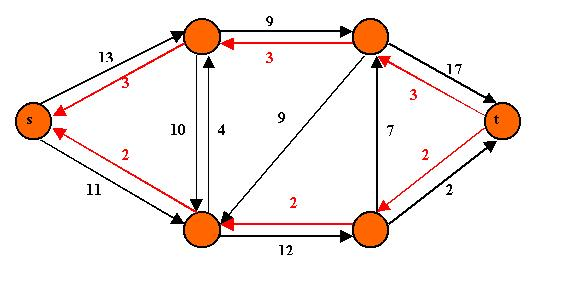
\includegraphics[width=0.5\textwidth]{./dados/figuras/figura1}
    \fonte{\citeonline{IRL2014}}
    \label{fig:figura-exemplo1}
\end{figure}

% EQUAÇÕES-----------------------------------------------------------------------
\chapter{EQUAÇÕES}
\label{chap:equacoes}

Exemplo de como inserir equações no corpo do texto \footnote{Deve-se atentar ao fato de a formatação das equações ficar muito boa esteticamente.}. Para adicionar uma equação inline, há três formas: 

\verb|\(E=mc^2\)| - Usando parênteses \verb|\(\)| = \(E=mc^2\)

\verb|$E=mc^2$| - Usando 1 cifrão antes e 1 depois = $E=mc^2$

Com a área math.
\begin{verbatim}
    \begin{math}
    E=mc^2
    \end{math}
\end{verbatim}

\begin{math}
    E=mc^2
\end{math}

Para adicionar uma equação display, há três formas:

\verb|\[E=mc^2\]| - Usando colchetes \verb|\[\]|
\[E=mc^2\]

\verb|$$E=mc^2$$| - Usando 2 cifrões antes e 2 depois
$$E=mc^2$$

E com o uso do ambiente \textit{equation} do pacote \textit{amsmath}.

\begin{verbatim}
    \begin{equation}
    X(s) = \int\limits_{t = -\infty}^{\infty} x(t) \, \text{e}^{-st} \, dt
    \label{eq:equacao-exemplo1}
    \end{equation}
\end{verbatim}

\begin{equation}
    X(s) = \int\limits_{t = -\infty}^{\infty} x(t) \, \text{e}^{-st} \, dt
    \label{eq:equacao-exemplo1}
\end{equation}

\begin{equation}
    F(u, v) = \sum_{m = 0}^{M - 1} \sum_{n = 0}^{N - 1} f(m, n) \exp \left[ -j 2 \pi \left( \frac{u m}{M} + \frac{v n}{N} \right) \right]
    \label{eq:equacao-exemplo2}
\end{equation}

% ALGORITMOS-----------------------------------------------------------------------
\chapter{ALGORITMOS}
\label{chap:algoritmos}

Exemplo de como inserir um algoritmo. Para inserção de algoritmos utiliza-se o pacote {\ttfamily algorithm2e} que já está devidamente configurado dentro do template.

Os algoritmos devem ser criados em arquivos separados para facilitar manutenção e armazenados no diretório de "/dados".\\
\\

\begin{algorithm}
    \caption{Exemplo de Algoritmo}
    \Entrada{o número $n$ de vértices a remover, grafo original $G(V, E)$}
    \Saida{grafo reduzido $G'(V,E)$}
    $removidos \leftarrow 0$ \\
    \While {removidos $<$ n } {
        $v \leftarrow$ Random$(1, ..., k) \in V$ \\
            \Repita {$u \in adjacentes(v)$} {
                remove aresta (u, v)\\
                $removidos \leftarrow removidos + 1$\\
            }
            \Se {há  componentes desconectados} {
                remove os componentes desconectados\\
            }
        }
\end{algorithm}


% SOBRE AS LISTAS--------------------------------------------------------------------
\chapter{SOBRE AS LISTAS}
\label{chap:apSobreLista}

Para construir listas de "\textit{bullets}"{} ou listas enumeradas, inclusive listas aninhadas, é utilizado o pacote \verb|paralist|.

Exemplo de duas listas não numeradas aninhadas, utilizando o comando \verb|\itemize|. Observe a indentação, bem como a mudança automática do tipo de "\textit{bullet}"{} nas listas aninhadas.

\begin{itemize}
    \item item não numerado 1
    \item item não numerado 2
    \begin{itemize}
        \item subitem não numerado 1
        \item subitem não numerado 2
        \item subitem não numerado 3
    \end{itemize}
    \item item não numerado 3
\end{itemize}

Exemplo de duas listas numeradas aninhadas, utilizando o comando \verb|\enumerate|. Observe a numeração progressiva e indentação das listas aninhadas.

\begin{enumerate}
    \item item numerado 1
    \item item numerado 2
    \begin{enumerate}
        \item subitem numerado 1
        \item subitem numerado 2
        \item subitem numerado 3
    \end{enumerate}
    \item item numerado 3
\end{enumerate}

% SOBRE AS CITAÇÕES E CHAMADAS DE REFERÊNCAS----------------------------------------------
\chapter{SOBRE AS CITAÇÕES E CHAMADAS DE REFERÊNCAS}
\label{chap:apSobreCita}

Citações são trechos de texto ou informações obtidas de materiais consultadss quando da elaboração do trabalho. São utilizadas no texto com o propósito de esclarecer, completar e embasar as ideias do autor. Todas as publicações consultadas e utilizadas (por meio de citações) devem ser listadas, obrigatoriamente, nas referências bibliográficas, para preservar os direitos autorais. São classificadas em citações indiretas e diretas.

% CITAÇÕES INDIRETAS-----------------------------------------------------------------------
\chapter{CITAÇÕES INDIRETAS}
\label{chap:citacoesLivres}

É a transcrição, com suas próprias palavras, das idéias de um autor, mantendo-se o sentido original. A citação indireta é a maneira que o pesquisador tem de ler, compreender e gerar conhecimento a partir do conhecimento de outros autores. Quanto à chamada da referência, ela pode ser feita de duas maneiras distintas, conforme o nome do(s) autor(es) façam parte do seu texto ou não. Exemplo de chamada fazendo parte do texto:\\
\\Enquanto \citeonline{Maturana2003} defendem uma epistemologia baseada na biologia. Para os autores, é necessário rever \ldots.\\

A chamada de referência foi feita com o comando \verb|\citeonline{chave}|, que produzirá a formatação correta.

A segunda forma de fazer uma chamada de referência deve ser utilizada quando se quer evitar uma interrupção na sequência do texto, o que poderia, eventualmente, prejudicar a leitura. Assim, a citação é feita e imediatamente após a obra referenciada deve ser colocada entre parênteses. Porém, neste caso específico, o nome do autor deve vir em caixa alta, seguido do ano da publicação. Exemplo de chamada não fazendo parte do texto:\\
\\Há defensores da epistemologia baseada na biologia que argumentam em favor da necessidade de \ldots \cite{Maturana2003}.\\

Nesse caso a chamada de referência deve ser feita com o comando \verb|\cite{chave}|, que produzirá a formatação correta.

% CITAÇÕES DIRETAS-----------------------------------------------------------------------
\chapter{CITAÇÕES DIRETAS}
\label{chap:citacoesLiterais}

É a transcrição ou cópia de um parágrafo, de uma frase, de parte dela ou de uma expressão, usando exatamente as mesmas palavras adotadas pelo autor do trabalho consultado.

Quanto à chamada da referência, ela pode ser feita de qualquer das duas maneiras já mencionadas nas citações indiretas, conforme o nome do(s) autor(es) façam parte do texto ou não. Há duas maneiras distintas de se fazer uma citação direta, conforme o trecho citado seja longo ou curto.

Quando o trecho citado é longo (4 ou mais linhas) deve-se usar um parágrafo específico para a citação, na forma de um texto recuado (4 cm da margem esquerda), com tamanho de letra menor e espaçamento entrelinhas simples. Exemplo de citação longa:
\\\begin{citacao}
    Desse modo, opera-se uma ruptura decisiva entre a reflexividade filosófica, isto é a possibilidade do sujeito de pensar e de refletir, e a objetividade científica. Encontramo-nos num ponto em que o conhecimento científico está sem consciência. Sem consciência moral, sem consciência reflexiva e também subjetiva. Cada vez mais o desenvolvimento extraordinário do conhecimento científico vai tornar menos praticável a própria possibilidade de reflexão do sujeito sobre a sua pesquisa \cite[p.~28]{Silva2000}.
\end{citacao}

Para fazer a citação longa deve-se utilizar os seguintes comandos:
\begin{verbatim}
\begin{citacao}
<texto da citacao>
\end{citacao}
\end{verbatim}

No exemplo acima, para a chamada da referência o comando \verb|\cite[p.~28]{Silva2000}| foi utilizado, visto que os nomes dos autores não são parte do trecho citado. É necessário também indicar o número da página da obra citada que contém o trecho citado.

Quando o trecho citado é curto (3 ou menos linhas) ele deve inserido diretamente no texto entre aspas. Exemplos de citação curta:\\
\\A epistemologia baseada na biologia parte do princípio de que "assumo que não posso fazer referência a entidades independentes de mim para construir meu explicar" \cite[p.~35]{Maturana2003}.\\
\\A epistemologia baseada na biologia de \citeonline[p.~35]{Maturana2003} parte do princípio de que "assumo que não posso fazer referência a entidades independentes de mim para construir meu explicar".

% DETALHES SOBRE AS CHAMADAS DE REFERÊNCIAS---------------------------------------------------------
\chapter{DETALHES SOBRE AS CHAMADAS DE REFERÊNCIAS}
\label{chap:referUtilizadas}

Outros exemplos de comandos para as chamadas de referências e o resultado produzido por estes:\\
\\\citeonline{Maturana2003} \ \ \  \verb|\citeonline{Maturana2003}|\\
\citeonline{Barbosa2004} \ \ \   \verb|\citeonline{Barbosa2004}|\\
\cite[p.~28]{Silva2000} \ \ \  \verb|\cite[p.~28]{Silva2000}|\\
\citeonline[p.~33]{Silva2000} \ \ \   \verb|\citeonline[p.~33]{v}|\\
\cite[p.~35]{Maturana2003} \ \ \   \verb|\cite[p.~35]{Maturana2003}|\\
\citeonline[p.~35]{Maturana2003} \ \ \   \verb|\citeonline[p.~35]{Maturana2003}|\\
\cite{Barbosa2004,Maturana2003} \ \ \   \verb|\cite{Barbosa2004,Maturana2003}|\\

% SOBRE AS REFERÊNCIAS BIBLIOGRÁFICAS-------------------------------------------------------
\chapter{SOBRE AS REFERÊNCIAS BIBLIOGRÁFICAS}
\label{chap:apSobreRefer}

A bibliografia é feita no padrão \textsc{Bib}\TeX{}. As referências são colocadas em um arquivo separado. Neste template as referências são armazenadas no arquivo "base-referencias.bib".

Existem diversas categorias documentos e materiais componentes da bibliografia. A classe abn\TeX{} define as seguintes categorias (entradas):

\begin{verbatim}
@book
@inbook
@article
@phdthesis
@mastersthesis
@monography
@techreport
@manual
@proceedings
@inproceedings
@journalpart
@booklet
@patent
@unpublished
@misc
\end{verbatim}

Cada categoria (entrada) é formatada pelo pacote \citeonline{abnTeX22014d} de uma forma específica. Algumas entradas foram introduzidas especificamente para atender à norma \citeonline{NBR6023:2002}, são elas: \verb|@monography|, \verb|@journalpart|,\verb|@patent|. As demais entradas são padrão \textsc{Bib}\TeX{}. Para maiores detalhes, refira-se a \citeonline{abnTeX22014d}, \citeonline{abnTeX22014b}, \citeonline{abnTeX22014c}.

% NOTAS DE RODAPÉ--------------------------------------------------------------------------
\chapter{NOTAS DE RODAPÉ}
\label{chap:notasRodape}

As notas de rodapé pode ser classificadas em duas categorias: notas explicativas\footnote{é o tipo mais comum de notas que destacam, explicam e/ou complementam o que foi dito no corpo do texto, como esta nota de rodapé, por exemplo.} e notas de referências. A notas de referências, como o próprio nome ja indica, são utilizadas para colocar referências e/ou chamadas de referências sob certas condições.
                   % Capítulo com Orientações de uso do Template
% CONCLUSÃO--------------------------------------------------------------------

\chapter{CONCLUSÃO}
\label{chap:conclusao}

Parte final do texto, na qual se apresentam as conclusões do trabalho acadêmico. É importante fazer uma análise crítica do trabalho, destacando os principais resultados e as contribuições do trabalho para a área de pesquisa.

\section{TRABALHOS FUTUROS}
\label{sec:trabalhosFuturos}

Também deve indicar, se possível e/ou conveniente, como o trabalho pode ser estendido ou aprimorado.

\section{CONSIDERAÇÕES FINAIS}
\label{sec:consideracoesFinais}

Encerramento do trabalho acadêmico.
                 			           % Conclusão

\postextual
% INSERE ELEMENTOS PÓS-TEXTUAIS
% REFERÊNCIAS------------------------------------------------------------------

% Carrega o arquivo "base-referencias.bib" e extrai automaticamente as referências citadas

\bibliography{./base-referencias}
\bibliographystyle{abntex2-alf} % Define o estilo ABNT para formatar a lista de referências
% OBSERVAÇÕES------------------------------------------------------------------
% Este arquivo não precisa ser alterado.
           			           % Referências
% APÊNDICES--------------------------------------------------------------------

\begin{apendicesenv}
\partapendices

% Primeiro apêndice------------------------------------------------------------
\chapter{Nome do apêndice} % Edite para alterar o título deste apêndice
\label{chap:apendiceA}

Lembre-se que a diferença entre apêndice e anexo diz respeito à autoria do texto e/ou material ali colocado.

Caso o material ou texto suplementar ou complementar seja de sua autoria, então ele deverá ser colocado como um apêndice. Porém, caso a autoria seja de terceiros, então o material ou texto deverá ser colocado como anexo.

Caso seja conveniente, podem ser criados outros apêndices para o seu trabalho acadêmico. Basta recortar e colar este trecho neste mesmo documento. Lembre-se de alterar o "label"{} do apêndice.

Não é aconselhável colocar tudo que é complementar em um único apêndice. Organize os apêndices de modo que, em cada um deles, haja um único tipo de conteúdo. Isso facilita a leitura e compreensão para o leitor do trabalho.

% Novo apêndice----------------------------------------------------------------
\chapter{Nome do outro apêndice}
\label{chap:apendiceB}

conteúdo do novo apêndice

\end{apendicesenv}
             			           % Apêndices
% ANEXO------------------------------------------------------------------------

\begin{anexosenv}
\partanexos

% Primeiro anexo---------------------------------------------------------------
\chapter{Nome do anexo}     % edite para alterar o título deste anexo
\label{chap:anexoA}

Lembre-se que a diferença entre apêndice e anexo diz respeito à autoria do texto e/ou material ali colocado.

Caso o material ou texto suplementar ou complementar seja de sua autoria, então ele deverá ser colocado como um apêndice. Porém, caso a autoria seja de terceiros, então o material ou texto deverá ser colocado como anexo.

Caso seja conveniente, podem ser criados outros anexos para o seu trabalho acadêmico. Basta recortar e colar este trecho neste mesmo documento. Lembre-se de alterar o "label"{} do anexo.

Organize seus anexos de modo a que, em cada um deles, haja um único tipo de conteúdo. Isso facilita a leitura e compreensão para o leitor do trabalho. É para ele que você escreve.

% Novo anexo-------------------------------------------------------------------
\chapter{Nome do outro anexo}
\label{chap:anexoB}

conteúdo do outro anexo

\end{anexosenv}
               			           % Anexos

\end{document}
